\documentclass{article}
\usepackage[utf8]{inputenc}
\usepackage{hyperref}
\usepackage[square,numbers]{natbib}
\usepackage{graphicx}
\usepackage{amsmath}
\usepackage{amssymb, graphics, setspace, mathtools}
\bibliographystyle{abbrvnat}

\title{Master Thesis Outline TQET33 \\
\normalsize{The Institute of Technology at Linköping University}}


\author{Maja Gasslander \\ \normalsize{maja.gasslander@gmail.com}}

%\date{November 16, 2015}

\begin{document}

\maketitle
\newpage
\section{Introduction}
This Master thesis will be carried out at Vricon. Supervisor at Vricon is Anton Nordmark, supervisor at ISY is Martin Danelljan and the examiner is Fahad Khan at ISY. 

\subsection{Contact Information}
Anton Nordmark: \href{mailto:anton.nordmark@vricon.com}{anton.nordmark@vricon.com}\\
Martin Danelljan: \href{mailto:martin.danelljan@liu.se}{martin.danelljan@liu.se} \\
Fahad Khan: \href{mailto:fahad.khan@liu.se}{fahad.khan@liu.se}


\section{Preliminary Title}
A preliminary title for the master thesis is \emph{Texture and Color based Classification of Clouds in Satellite Images using SVM.} 

\section{Problem Formulation}
The aim of the thesis is to evaluate methods to segment satellite images into cloud and non-cloud pixels, and compare the result to Vricon's inhouse methods. Different combinations of existing methods for feature extraction and classification will be evaluated.

\section{Approach}
A preliminary approach for solving the task is to divide the problem into several smaller problems. Each subproblem is described in more detail in the subsections below. The pipeline can be seen in figure \ref{fig:pipeline} below.

\begin{figure}[h!]
    \centering
    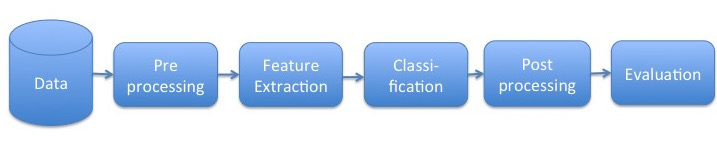
\includegraphics[scale=0.5]{fig/pipeline}
    \caption{Pipeline}
    \label{fig:pipeline}
\end{figure}

\subsection{Data}
The images that will be used for cloud classification in this thesis is both panchromatic high resolution images, and also an eight-band multispectral imagery, containing various types of landscape and cloud amount. All images will be provided by Vricon.

\subsection{Pre processing}
To make the classification easier the images are pre processed. This will be done by tiling the images into smaller tiles. An alternative to tiling is to do a superpixel segmentation that will be taken into consideration. Also, a histogram equalization will be applied. This will flatten the greylevel histogram of the image so that all intensities are as equal as possible and thereby the image contrast is increased.

%\subsubsection{Tiling}
%First the image $I$ is divided into smaller tiles, $I_k$. To avoid wrong classification in the tiles containing cloud boundaries, overlapping tiles is used. 

%\subsubsection{Edge detection}
%Since clouds contains very little sharp edges, many of the non-cloud tiles can be sorted away by calculating the edges with the canny edge detector \citep{canny}.

%\subsubsection{Histogram Equalization}

\subsection{Feature Extraction}
After the pre processing is done it is time to perform the feature extraction. A good feature clearly seperates the two classes from each other. Texture and color are the two features that will recieve the biggest focus. Some suggestions for features extractions to test are:

\begin{itemize}
\item Gabor Filters: \\
A set of Gabor filters with different frequencies and orientation might be good to extract  texture features from the clouds.
The equation for a complex Gabor filter looks like follows:
\begin{equation}
g(x, y; \lambda, \theta, \psi, \sigma, \gamma) = e^{-\frac{x'^2 + \gamma^2y'^2}{2\sigma^2}}e^{i(2\pi\frac{x'}{\lambda} + \psi)}
\end{equation}
where \\
$x' = x\cos\theta + y\sin\theta$ \\
and \\
$y' = -x\sin\theta + y\cos\theta$

\item Homogeneous Texture Descriptor: \\
Clouds have a very homogeneous texture, so the Homogeneous Texture Descriptor (HTD) might be good to extract texture features in the clouds. 

\item Grey level co-occurrence matrix: \\
A grey level co-occurrence matrix (GLCM) is a histogram of co-occurring greyscale values at a given offset over an image. The GLCM functions characterize the texture of an image by calculating how often pairs of pixels with specific values and in a specified spatial relationship occur in an image.

\item Color: \\
Since the clouds often differ in color compared to other areas with simliar texture (for example water) it might be good to use color as an feature for the classification. 
\end{itemize}
Additional features that is discovered during the work might be tested as well.

%\subsubsection{Homogeneous Texture Descriptor}

%\subsubsection{Grey level co-occurrence matrix}

%\subsubsection{Color}

\subsection{Classification}
Then it is time to do the actual classification. This is done by Support Vector Machines (SVM) which is a supervised learning method. 
Consider a set of \textit{training} vectors $ \textbf{x}_{i}, i = 1,...,k $, which are the feature vectors, and the corresponding vector $ \textbf{y} $ of length $ k $ containing the class values; 

\begin{equation}
y_{i} =
\begin{cases}
1, & \text{if $\textbf{x}_{i}$ in class 1} \\
-1,
& \text{if $\textbf{x}_{i}$ in class 2}
\end{cases}
\end{equation}
Then we have the separating hyperplane as $\textbf{w}^{T}\textbf{x} + b = 0$

\begin{equation}
\label{eq:hyp}
\begin{cases}
(\textbf{w}^{T}\textbf{x}_{i}) + b > 0 & \text{if $y_{i} = 1$} \\
(\textbf{w}^{T}\textbf{x}_{i}) + b < 0 & \text{if $y_{i} = -1$}
\end{cases}
\end{equation}

The decision function then becomes $f(\textbf{x}) = sgn(\textbf{w}^{T}\textbf{x} + b)$, where $ \textbf{x} $ is the testdata. There are many possible choices for $\textbf{w}$ and $b$.
Equation \ref{eq:hyp} can be rewritten as 

\begin{equation}
y_{i}(\textbf{w}^{T}\textbf{x}_{i} + b) \geq 1, \text{for all $1 \leq i \leq k$}
\end{equation}

which gives an optimization problem: \\

\begin{equation}
\min_{\textbf{w},b} \dfrac{1}{2}\textbf{w}^{T}\textbf{w}
\end{equation}

subject to (for any $ i = 1,...,k $)

\begin{equation*}
y_{i}(\textbf{w}^{T}\textbf{x}_{i} + b) \geq 1
\end{equation*}

If the data is not linearly seperable it can be mapped to a higher dimensional feature space using the Kernel trick: $ K(\textbf{x}_{i},\textbf{x}_{j}) = \phi(\textbf{x}_{i})^{T}\phi(\textbf{x}_{j}) $ \\
where
\begin{equation*}
\phi(\textbf{x}_{i}) = (\phi_{1}(\textbf{x}_{i}), \phi_{2}(\textbf{x}_{i}),...)
\end{equation*}
The new equation is:

\begin{equation}
\min_{\textbf{w},b, \xi} \dfrac{1}{2}\textbf{w}^{T}\textbf{w} + C\sum_{1 = 1}^{k}\xi_{i}
\end{equation}
\begin{equation*}
\xi_{i} \geq 0, i = 1,...,k
\end{equation*}
subject to (for any $ i = 1,...,k $)

\begin{equation*}
y_{i}(\textbf{w}^{T}\phi(\textbf{x}_{i}) + b) \geq 1 - \xi_{i}
\end{equation*}
Some common kernels that will be tested during this thesis are: \\
\begin{itemize}
\item Linear Kernel: $K(\textbf{x}_i,\textbf{x}_{j}) = \textbf{x}_i\cdot\textbf{x}_{j}$

\item Polynomial Kernel: $K(\textbf{x}_i,\textbf{x}_{j}) = (\gamma\textbf{x}_i\cdot\textbf{x}_{j} + r)^d, \gamma > 0$

\item Gaussian Radial Basis Function: $K(\textbf{x}_i,\textbf{x}_{j}) = e^{(-\gamma\|\textbf{x}_i-\textbf{x}_{j}\|)^2}, \gamma > 0$

\item Sigmoid Kernel: $K(\textbf{x}_i,\textbf{x}_{j}) = \tanh(\gamma\textbf{x}_i\cdot\textbf{x}_{j} + r)$
\end{itemize}

\subsection{Post processing}

After the classification is done some post processing might need to be implemented to clean up some of the wrongly classified objects. For example a shape based post processing can be used to remove objects that are to "perfect" from the cloud class.

\subsection{Evaluation}
When the classification is done the result needs to be evaluated to know how the algorithm performed. This will be done by comparing the classified images to a hand labeled ground truth. Some ground truth already exists, and some might need to be hand labeled during the thesis. 

\section{Time Plan}
The given task has been divided into several sub tasks to easier plan the work. The estimated time for each sub task is listed in the time plan in figure \ref{fig:timeplan} below.
Note that week 53-2 and week 11-12 are marked red because of Christmas break and exams.

%\subsection{Activities}
%\begin{itemize}
%\item Literature study.
%\item Preparatory work.
%item Preprocessing
%item Feature extraction texture
%\item Feature extraction color
%\item Classification
%\item Evaluation
%\item Documentation
%\item Presentation
%\item Opposition
%\item Meetings supervisor
%\end{itemize}

\subsection{Dates}
\begin{itemize}
\item Half-time Control: February 3, 2016.
\item Presentation: April 20, 2016.
\end{itemize}

\begin{figure}[h!]
    \centering
    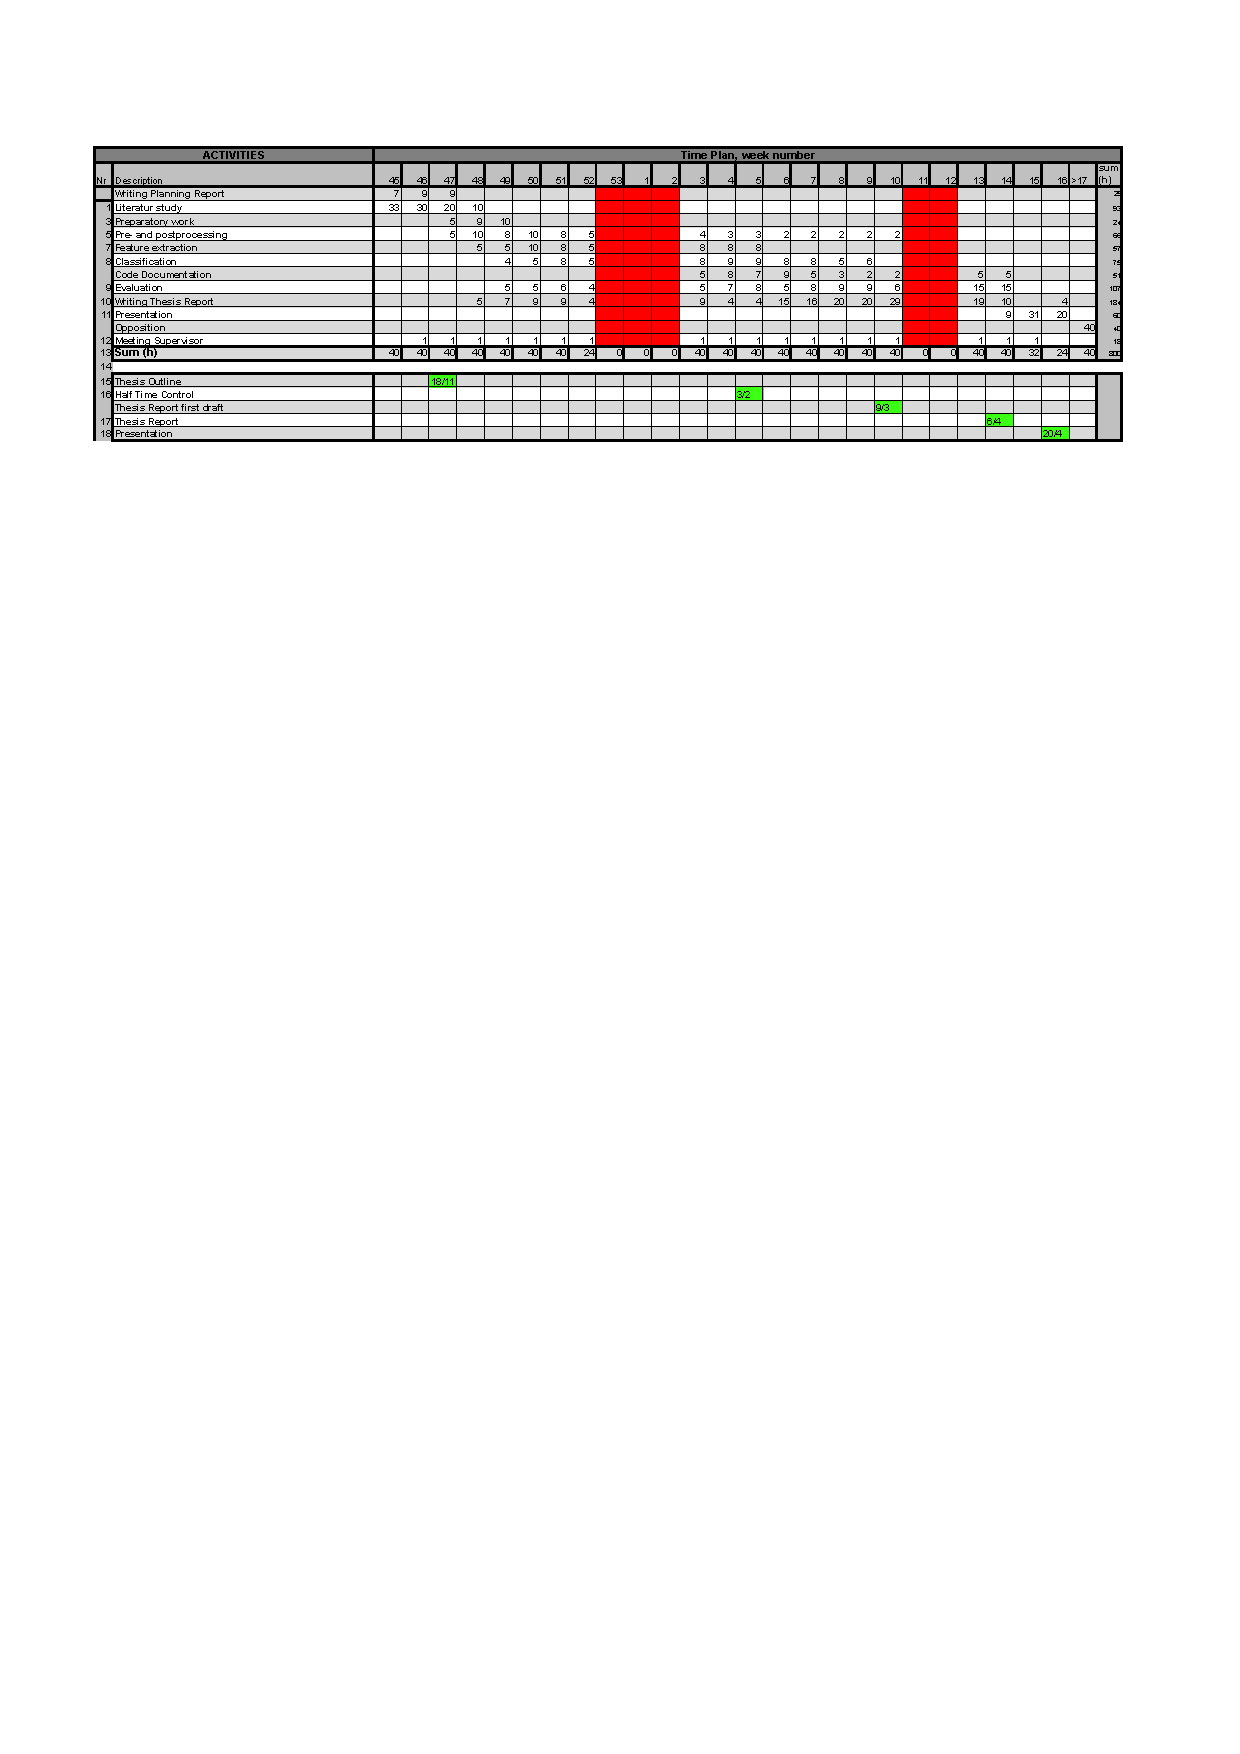
\includegraphics[height=9 cm, width=18 cm, angle=90]{fig/Tidplan}
    \caption{Time Plan}
    \label{fig:timeplan}
\end{figure}

\newpage

\section{Literature}
\renewcommand{\section}[2]{}%
\begin{thebibliography}{9}

\bibitem{cloudcolor} 
Emre Ba\c{s}eski and \c{C}a\v{g}lar \c{S}enaras. 
\textit{Texture and Color Based Cloud Detection.}
HAVELSAN A.S., 2015.
 
\bibitem{cloudtexture} 
H.K. Chethan, R. Raghavendra and G. Kumar Hemantha. 
\textit{Texture based Approach for Cloud Classification using SVM.} \\
International Conference on Advances in Recent Technologies in Communication and Computing, 2009. 
 
\bibitem{canny} 
J. Canny. 
\textit{A computational Approach to Edge Detection.} \\
IEEE Transactions on Pattern Analysis and Machine Intelligence, 1986. 
 
\bibitem{woods} 
Rafael C. Gonzales and Richard E. Woods. 
\textit{Digital Image Processing.} \\
Pearson Education, Inc., 2008.
 
\bibitem{gabor} 
D. Zheng, Y. Zhao and j. Wang. 
\textit{Feature Extraction using a Gabor Filter Family.} \\
Proceedings of the 6th IASTED International Conference, Signal and Image Processing, 2004. 

\bibitem{programming} 
Jan Erik Solem. 
\textit{Programming Computer Vision with Python.} \\
Creative Commons, 2004.

\bibitem{htd} 
Y. Man Ro, M. Kim, H.K. Kang, B.S. Manjunath and J. Kim
\textit{MPEG-7 Homogeneous Texture Descriptor.} \\
ETRI Journal, volume 23, Number 2, 2001. 

\bibitem{svm} 
A. Ben-Hur and J. Weston
\textit{A User's Guide to Support Vector Machines.} \\
ETRI Journal, volume 23, Number 2, 2001. 

%\bibitem{knuthwebsite} 
%Knuth: Computers and Typesetting,
%\\\texttt{http://www-cs-faculty.stanford.edu/\~{}uno/abcde.html}
\end{thebibliography}

%\bibliography{bibfile}
\end{document}
